\documentclass[12pt,a4paper]{article}
\usepackage[utf8]{inputenc}
\usepackage[OT1]{fontenc}
\usepackage{amsmath}
\usepackage{amsfonts}
\usepackage{amssymb}
\usepackage{graphicx}
\usepackage{tikz}
\usepackage{pgfplotstable}
\usepackage{mathtext}

\usepackage[T1]{fontenc}
\usepackage[utf8]{inputenc}
\usepackage[english, bulgarian, russian]{babel}

\usepackage{tikz}
\usepackage{pgfplots}
\usepackage{indentfirst}
\usepackage[export]{adjustbox}
\usepackage{multirow}
\usepackage{geometry} \geometry{verbose,a4paper,tmargin=2cm,bmargin=2cm,lmargin=1.5cm,rmargin=1.5cm}

\graphicspath{{Images/}}
\usepackage[left=2cm,right=2cm,top=2cm,bottom=2cm]{geometry}
\usepackage{wrapfig}
\usepackage{setspace}
\usepackage{indentfirst}
\usepackage{subfigure}


\begin{document}

\begin{titlepage}
  \begin{center}
    \huge
    Московский Физико-технический Институт
    
    (Национальный исследовательский университет)
    \vspace{0.5cm}

   
    \vspace{0.25cm}
 
    \vfill
 
    \vfill

    \textsc{\bf{Отчет выполнении работы 2.2.1}}\\[3mm]
    
    {\LARGE Исследование взаимной диффузии газов}
  \bigskip
    \vfill
    
\end{center}
\vfill
\begin{flushright}

    Выполнили студентки 1 курса
    
    ФБМФ, группа Б06-103

    Попеску Полина
    
    
    Фитэль Алёна

\end{flushright}
\bigskip


\vfill

\begin{center}
  Долгопрудный, 2022 г.
\end{center}
\end{titlepage}

\section{Введение}

\textbf{Цель работы:} 1)  регистрация  зависимости  концентрации   гелия в воздухе от времени с помощью датчиков теплопроводности при разных начальных давлениях смеси газов; 2) определение коэффициента диффузии по результатам измерений.

\textbf{В работе используются:} измерительная установка; форвакуумный насос; баллон с газом (гелий); манометр; источник питания; магазин сопротивлений; гальванометр; секундомер.

\section{Теоретические сведения}

Диффузия - самопроизвольное взаимное проникновение веществ друг в друга,  происходящее вследствие хаотичного теплового движения молекул.  
В системе, состоящей из двух компонентов,  плотность потока вещества в результате взаимной диффузии описывается законом Фика:
\begin{equation}
j_a = -D\frac{\partial n_a}{\partial x}, j_b = -D\frac{\partial n_b}{\partial x}
\end{equation}
где $D$ - коэффициент взаимной диффузии компонентов, $j_a$,  $j_b$ - плотности потока частиц соответствующего сорта (количество частиц, пересекающих единичную площадку в единицу времени).\\

В данной работе исследуется взаимная диффузия гелия и воздуха. Давление $P$ и температура $T$ в условиях опыта предполагаются неизменными:
$P = (n_{He}+n_{в})k_{Б},
T = const$, где $n_{He}$ и $n_{в}$
 — концентрации (объёмные плотности) диффундирующих газов. Поэтому для любых изменений концентраций справедливо $\delta n_{в}=−\delta n_{He}$. Следовательно, достаточно ограничиться описанием диффузии одного из компонентов, например гелия $n_{He}$.

Проведём теоретическую оценку величины коэффициента взаимной диффузии. В работа мала концентрация гелия, более того,  масса атомов гелия много меньше массы молекул, составляющих воздух, значит и их средняя тепловая скорость велика по сравнению с остальными частицами. Поэтому перемешивание газов в работе можно приближенно описывать как диффузию примеси лёгких частиц He на практически стационарном фоне воздуха. Коэффициент диффузии в таком приближении равен 
\begin{equation}
    D = \frac{1}{3}\lambda_{He} \bar v,
\label{eq:D}
\end{equation}
где $\lambda_{He} = \frac{1}{n_{\Sigma} \sigma}$, где $n_{\Sigma} = n_{He} + n_{в} = \frac{P}{k_{Б} T}$ - длина свободного пробега частиц гелия,  $\sigma$ -  среднее сечение столкновения частиц гелия с воздухом,  $\bar v = \sqrt{\frac{8kT}{\pi \mu}}$ - средняя тепловая скорость. 

Таким образом, теоретическая оценка предполагает, что коэффициент диффузии не зависит от пропорция элементов, а обратно пропорционален давлению $D \propto \frac{1}{P_\Sigma}$.\\

Рассмотрим подзадачу о диффузии в соединительной
трубке. Предположим сперва, что концентрации примеси
(гелия) на её торцах поддерживаются постоянными и
равными $n_{1}$ и $n_{2}$ соответственно. Тогда через некоторое время в трубке установится стационарный поток частиц, одинаковый в каждом сечении трубки (в противном случае, если бы поток зависел от x, частицы бы накапливались в трубке, и процесс перестал бы быть стационарным). Применяя закон Фика в трубке, получим

\begin{equation}
j = - D \frac{\partial n}{\partial x} = Const
\end{equation}

Следовательно,  распределение концентрации в трубке $n(x)$ - линейная функция:

\begin{equation}
n(x) = \frac{\Delta n}{L}x
\end{equation}

и плотность потока частиц всюду постоянна и равна

\begin{equation}
j = -D \frac{\Delta n}{L}
\end{equation}

где $\Delta n = n_{2} - n_{1}$ - разность концентраций гелия на концах трубки.

Так как процесс стационарный,  то справедливо:

\begin{equation}
\frac{dN_1}{dt} = jS,  \frac{dN_2}{dt} = -jS
\end{equation}

Тогда получаем:

\begin{equation}
\frac{d(\Delta n)}{t} = - \frac{\Delta n}{\tau},  \text{ где } \tau = \frac{1}{2} \frac{VL}{DS}
\label{eq:get_D_for_graph}
\end{equation}

Интегрируя,  получаем:

\begin{equation}
\Delta n = \Delta n_0 e ^{-t/\tau}
\label{eq:delta_n_exponenta}
\end{equation}

где $n_{0}$ — разность концентраций примеси в сосудах в начальный момент
времени

Так как $U \propto \Delta k \propto \Delta n$,  то:

\begin{equation}
U = U_{0} e^{-t/\tau}
\label{eq:u_exponenta}
\end{equation}

где $U_0$ — показание гальванометра в начальный момент времени.

	
\section{Экспериментальная установка}

\item Установка состоит из двух сосудов $V_1$ и $V_2$, соединённых краном $K_3$, форвакуумного насоса,  манометра М и системы напуска гелия, состоящей из кранов $K_6,  K_7$.  Кран $K_5$ позволяет соединять форвакуумный насос либо с установкой,  либо с атмосферой.  Сосуды $V_1$ и $V_2$ соединены трубкой длины $l$ и сечения $S$. Сосуды заполнены смесь двух газов при одинаковом давлении,  но с различной концентрацией компонентов.  Вследствие взаимной диффузии концентрации каждого из компонентов с течением времени выравниваются. Между форвакуумным насосом и краном $K_5$ вставлен предохранительный баллон, защищающий кран и установку при неправильной её эксплуатации от попадания форвакуумного масла из насоса.  Сосуды $V_1$ и $V_2$ можно соединять как с системой напуска гелия,  так и с форвакуумным насосом.  Для этот служат краны $K_1, K_2, K_4, K_5$.  Манометр М регистрирует давление газа,  до которого заполняют тот или иной сосуды. Кран $K_4$ изолирует форвакуумный насос от установки.  Для подачи воздуха в установку служит кран $K_5$. 

\begin{figure}[h!]
	\center{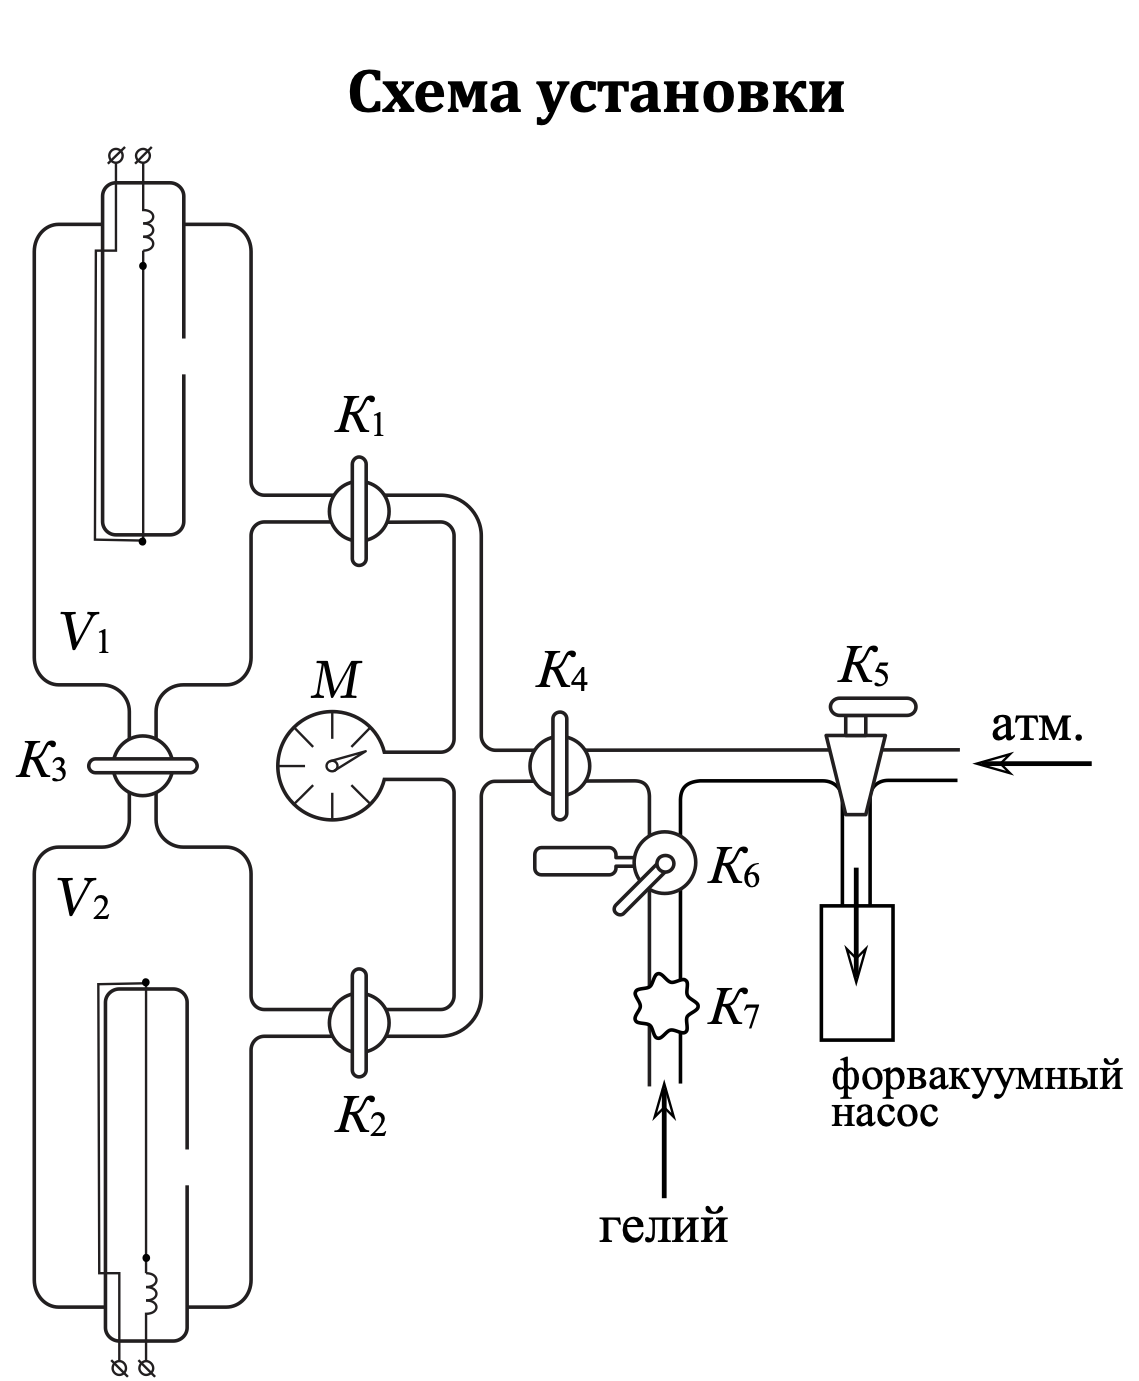
\includegraphics[scale=0.4]{ustanovka}}
\end{figure}

\item Для измерения разности концентраций газов используется мостовая схема.  Здесь $\text{Д}_1,  \text{Д}_2$ - датчики теплопроводности,  расположенные в сосудах $V_1$ и $V_2$.  Сопротивления $R_1,  R_2, R$ служат для  балансировка моста.  В одну из диагоналей моста включен гальванометр,  к другой подключается небольшое постоянное напряжение.  Сопротивления $R_1$ и $R_2$ спарены (их подвижные контакты находятся на общей оси) и изменяются одновременно при повороте ручки грубой регулировки. Точная балансировка выполняется потенциометром R.  

\begin{figure}[h!]
	\center{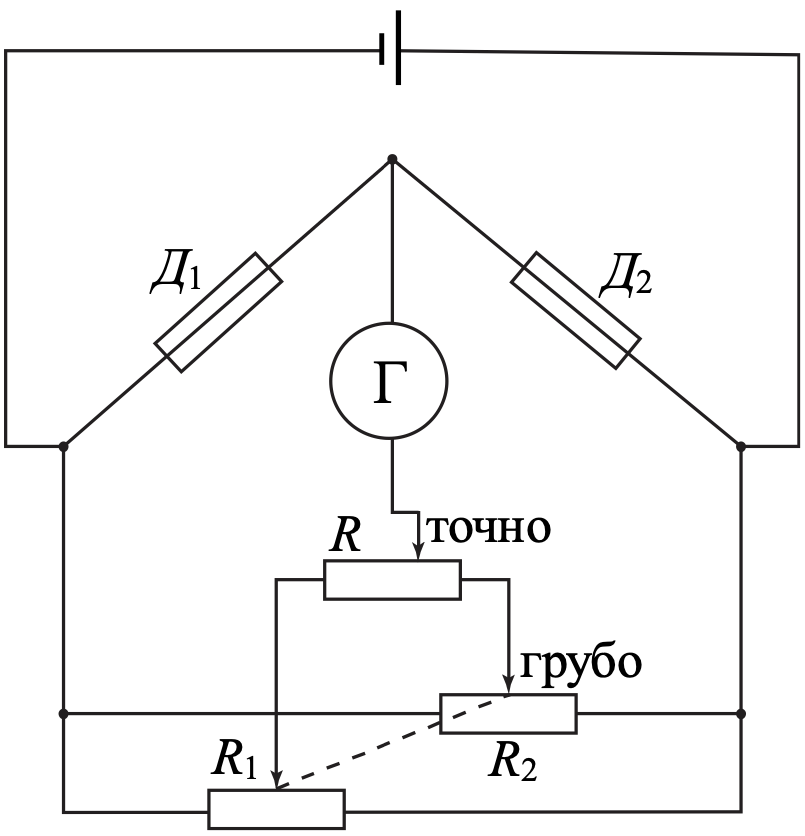
\includegraphics[scale=0.4]{most}}
\end{figure} 
 
\item Гелий содержится в баллоне под давлением,  превышающим атмосферное.  Для предотвращения избыточного расхода гелия и его неконтролируемого проникания в установку предусмотрен металлический кран ($К_7$),  отделяющий её от баллона с гелием.  Для подачи малых порций гелия предусмотрен двух-ходовый кран с дозатором.  

\begin{figure}[h!]
	\center{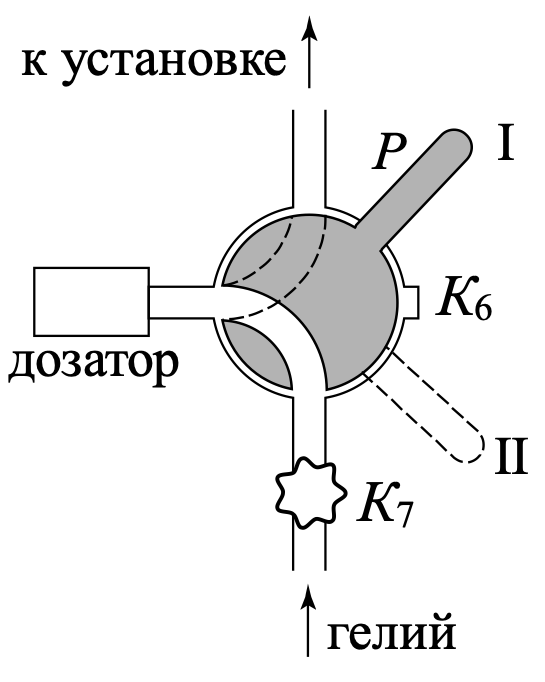
\includegraphics[scale=0.4]{dozator}}
\end{figure}

Параметры установки: $V_1 = V_2 = V = (775 \pm 10) \text{ см}^3$; $\frac{L}{S} = (5.3 \pm 0.1) \text{ см}^{-1}$.

	\section{Обработка результатов измерений}
\begin{enumerate}

\item Сбалансируем измерительный мост при предполагаемом «рабочем»
давлении.  
\item Заполним установку рабочей смесью: в сосуде $V_1$ находится воздух, а в сосуде $V_2$ - смесь воздуха с гелием.  Давление должно быть одинаковым и равным рабочему давлению $P_\Sigma$. 
\item Откроем кран $K_3$. Начнется процесс диффузии. Измерения будем продолжать до тех пор,  пока напряжение не упадет примерно на 50$\%$.
\item  Повторим измерения 5 раз при различных значениях рабочего давления.
\item Построим графики зависимостей изменений показания вольтметра от времени. Наблюдается экспоненциальная зависимость.

\begin{figure}[h!]
	\center{\includegraphics[scale=0.1]{U(t)graph221_1.png}}
\end{figure}

\item Построим графики зависимостей показаний вольтметра от времени в логарифмическом масштабе. 

\begin{figure}[h!]
	\center{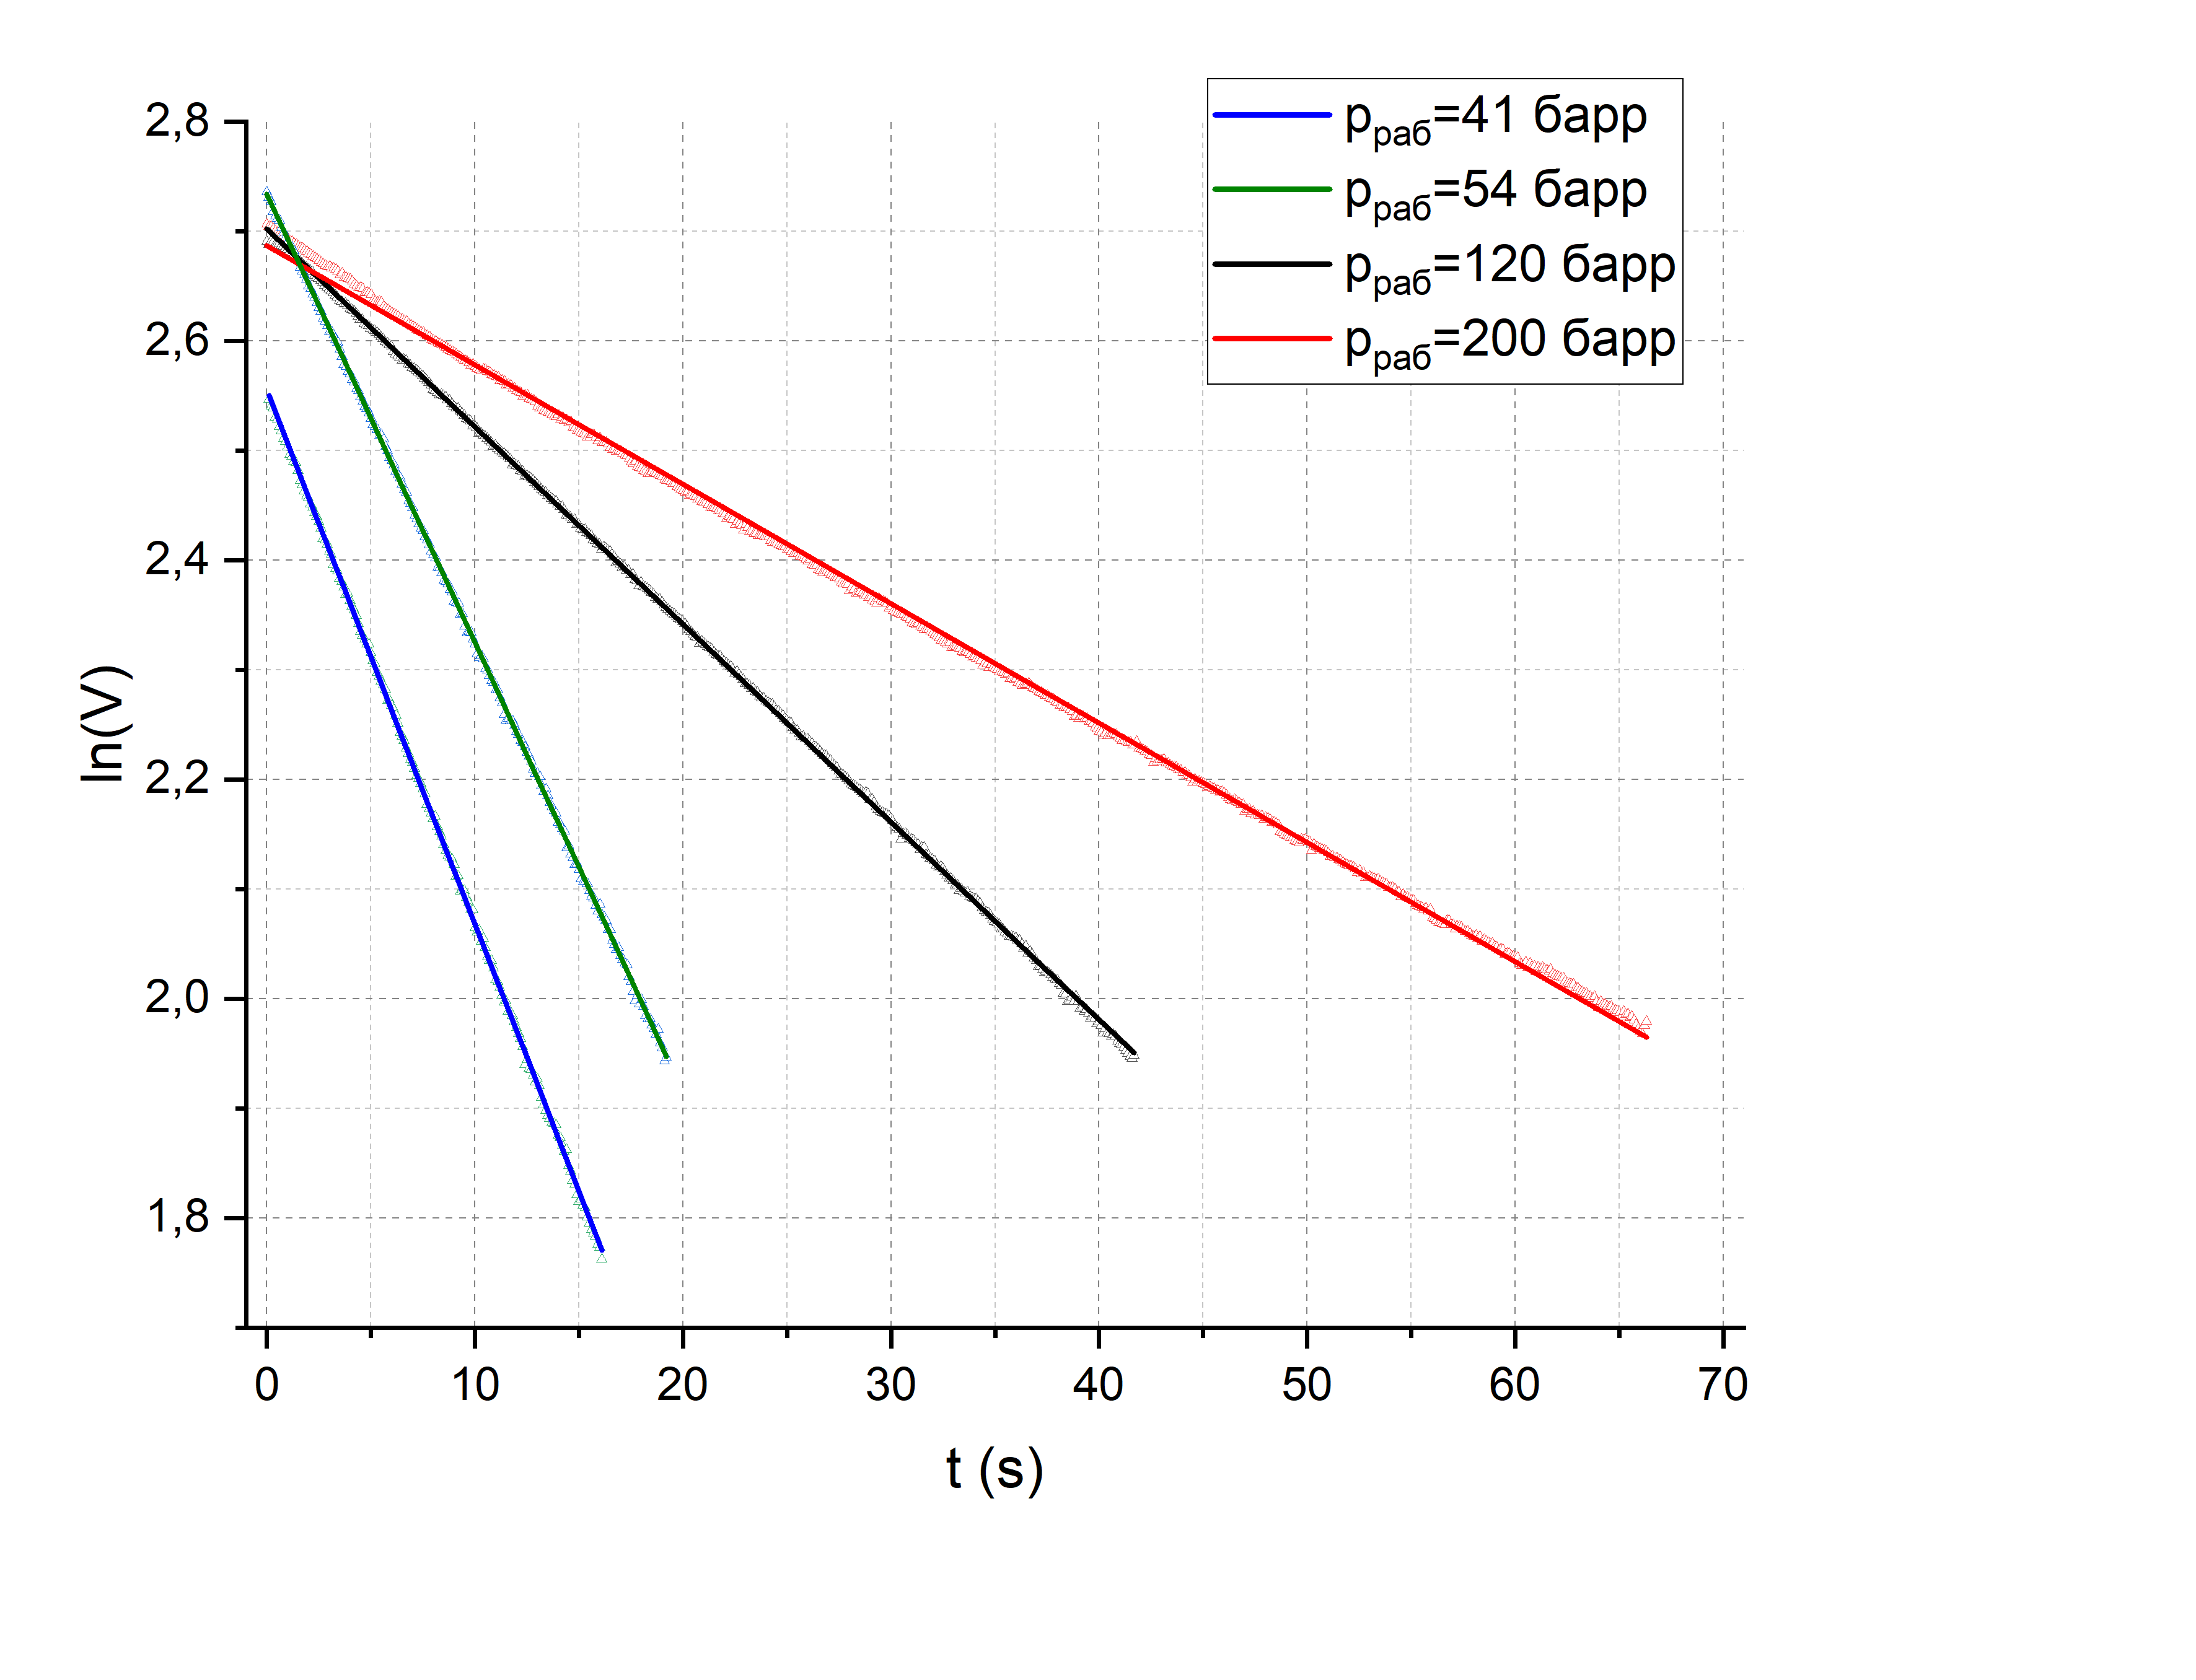
\includegraphics[scale=0.4]{lnU(t)graph221_2.png}}
\end{figure}

Рассчитаем коэффициент взаимной диффузии для различных значений рабочего давления.

Согласно формуле (\ref{eq:get_D_for_graph}): $$D = k \frac{VL}{2S}$$

$$\frac{\Delta D}{D} = \sqrt{\left(\frac{\Delta k}{k}\right)^2 + \left(\frac{\Delta V }{V}\right)^2 + \left(\frac{\Delta {L/S}}{L/S}\right)^2}, $$ где $k$ - коэффициент наклона прямой.

Таким образом, находим:

\begin{table}[h!]
\centering
\begin{tabular}{|c|c|c|c|c|}
\hline
$p$, барр         & 41    & 54    & 120   & 200   \\ \hline
$k, 10^{-3}$/с    & -4,87 & -4,09 & -1,8  & -1,09 \\ \hline
$\sigma_k, 10^{-3}$/с  & 0,006 & 0,003 & 0,001 & 0,001 \\ \hline
$D$, $10^{-4}$м$^2$/с & 10,00 & 8,40  & 3,70  & 2,24  \\ \hline
$\sigma_D$, м$^2$/с     & 0,29  & 0,25  & 0,11  & 0,07  \\ \hline
$p_0/p$            & 17,58 & 13,35 & 6,01  & 3,60  \\ \hline
$\sigma_{p_0/p}$         & 0,05  & 0,03  & 0,02  & 0,01  \\ \hline
\end{tabular}
\end{table}

\item Построим график зависимости коэффициента диффузии от обратного давления в координатах $D(\frac{P_0}{P})$. Экстраполируем график к атмосферному давлению,  оцениваем соответствующий коэффициент диффузии.

\begin{figure}[h!]
	\center{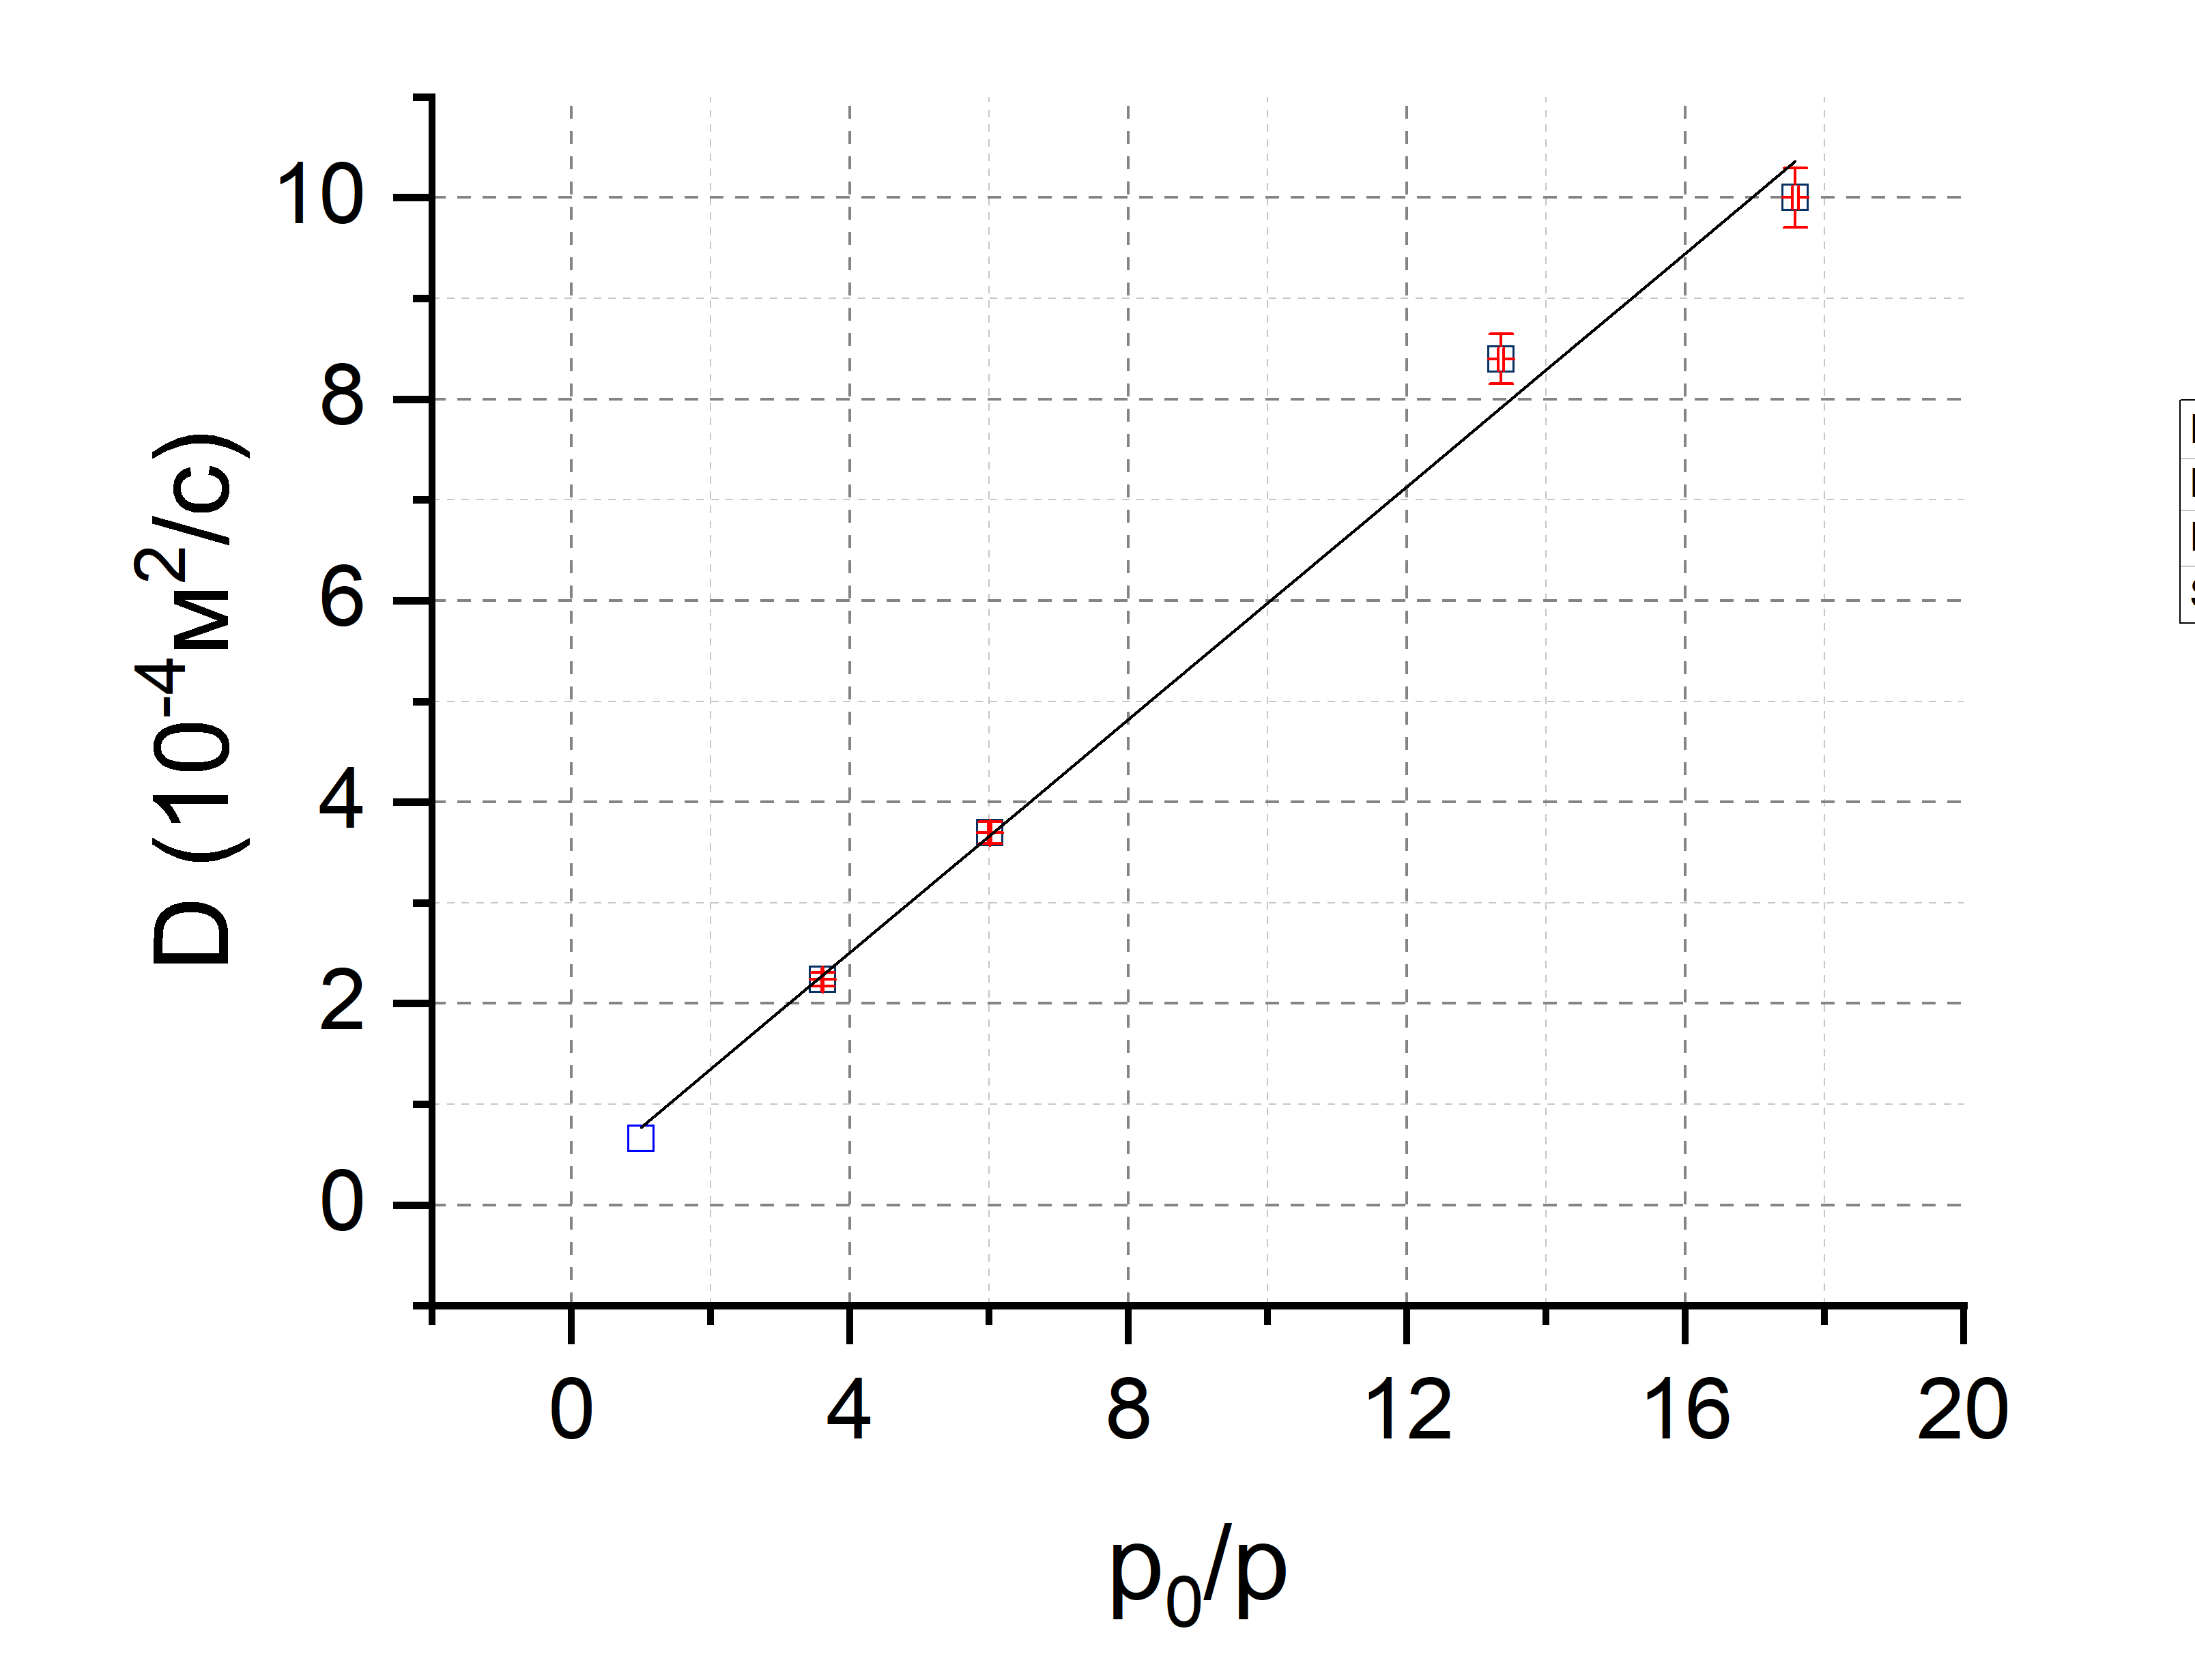
\includegraphics[scale=0.4]{D(p:p0)graph221_3.png}}
\end{figure}

Получаем $k = (0.58 \pm 0.03)$

Таким образом, для атмосферного давления в лаборатории ($P = 720,848$ торр)

\[D = (0.66 \pm 0.03) \frac{\text{см}^2}{\text{с}}\]

Табличное значение при атмосферном давлении: $D = 0,72 \frac{см^2}{с}$.

\item Оценим длину свободного пробега атомов гелия в воздухе $\lambda_{He}$.
 
$$D = \frac{1}{3} \lambda_{He} \bar v,\; где\;  \bar v = \sqrt{\frac{8RT}{\pi \mu}}$$

Отсюда получаем: 

$$\lambda_{He} = 3D \sqrt{\frac{\pi \mu}{8RT}} \approx (1.58\pm 0.07)  \cdot 10^{-7} \text{м}$$ 

$$
\frac{\Delta \lambda_{He}}{\lambda_{He}} =\sqrt{\left(\frac{\Delta D}{D}\right)^2+\frac{1}{4}\left(\frac{\Delta T}{T}\right)^2} \approx 4\%
$$

\item Оценим эффективное сечение столкновений атомов гелия с молекулами воздуха $\sigma$.

$$n_{\Sigma} = n_{He} + n_{в} = \frac{P_{\Sigma}}{k_Б T}, \sigma = \frac{1}{\lambda_{He} n_\Sigma} $$

$$\sigma = (2.62 \pm 0.12) \cdot 10^{-19} м^2$$ 

$$
\frac{\Delta \sigma}{\sigma} = \sqrt{\left(\frac{\Delta \lambda_{He}}{\lambda_{He}}\right)^2+\left(\frac{\Delta T}{T}\right)^2+\left(\frac{\Delta P_\Sigma}{P_{\Sigma}}\right)^2} \approx 5\%
$$

\end{enumerate}


\section{Вывод}

В данной работе было проверено, что закон $U = U_0 \cdot e^{\frac{-t}{\tau}}$ выполняется.

Был найден коэффициент диффузии гелия в воздухе. Измеренный коэффициент диффузии $D = (0.66 \pm 0.03)\cdot 10^{-4} \frac{\text{м}^2}{\text{с}}$ отличается от табличного $D_\text{табл} = 0.72 \frac{\text{м}^2}{\text{с}}$ на $ 9\% $. 

Кроме того, была оценена длина свободного пробега атомов гелия в воздухе и эффективное сечение столкновений атомов гелия с молекулами воздуха: $\lambda_{He} = (1.58\pm 0.07)  \cdot 10^{-7} \text{м}$, $\sigma = (2.62 \pm 0.12) \cdot 10^{-19} м^2$. Параметры системы могут сильно отличаться, поэтому сравнивать эти величины с табличными не получится.



\end{document}
